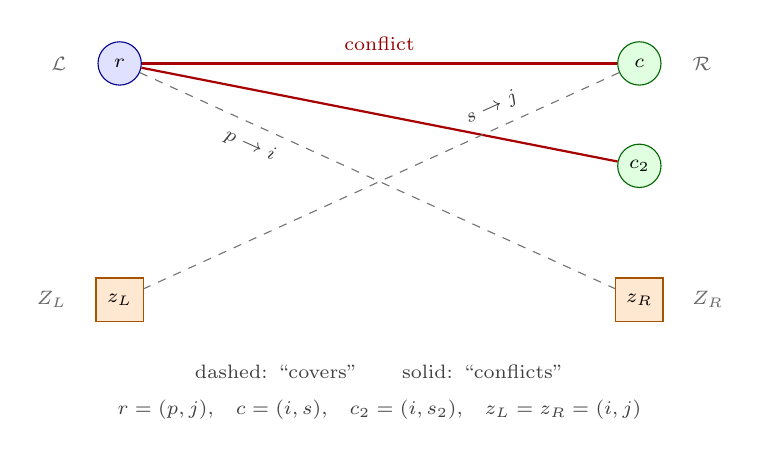
\begin{tikzpicture}[
  lv/.style={circle,draw=blue!55!black,fill=blue!12,minimum size=5.5mm,inner sep=0pt,font=\scriptsize},
  rv/.style={circle,draw=green!40!black,fill=green!12,minimum size=5.5mm,inner sep=0pt,font=\scriptsize},
  zv/.style={rectangle,draw=orange!65!black,fill=orange!18,minimum width=6mm,minimum height=5.5mm,inner sep=1pt,font=\scriptsize},
  conf/.style={draw=red!65!black,thick},
  cov/.style={draw=black!55,dashed},
  lab/.style={font=\scriptsize,text=black!75},
  grp/.style={font=\scriptsize\bfseries,text=black!60}
]
\node[lv] (r) at (0,3.2) {$r$};
\node[zv] (zl) at (0,0.2) {$z_L$};
\node[rv] (c) at (6.6,3.2) {$c$};
\node[rv] (c2) at (6.6,1.9) {$c_2$};
\node[zv] (zr) at (6.6,0.2) {$z_R$};
\node[grp,anchor=east] at (-0.55,3.2) {$\mathcal L$};
\node[grp,anchor=east] at (-0.55,0.2) {$Z_L$};
\node[grp,anchor=west] at (7.15,3.2) {$\mathcal R$};
\node[grp,anchor=west] at (7.15,0.2) {$Z_R$};
\draw[conf] (r) -- node[above=1pt,lab,text=red!60!black] {conflict} (c);
\draw[conf] (r) -- (c2);
\draw[cov] (c) -- node[near start,above=1pt,lab,sloped] {$s\to j$} (zl);
\draw[cov] (r) -- node[near start,below=1pt,lab,sloped] {$p\to i$} (zr);
\node[lab,anchor=north] at (3.3,-0.5) {dashed: ``covers''\qquad solid: ``conflicts''};
\node[lab,anchor=north] at (3.3,-0.95) {$r=(p,j)$,\quad $c=(i,s)$,\quad $c_2=(i,s_2)$,\quad $z_L=z_R=(i,j)$};
\end{tikzpicture}
